\documentclass{article}
\usepackage{graphicx}
\usepackage[toc,page]{appendix}

\begin{document}

\title{CS23710 Assignemnt}
\author{Samuel B Sherar (sbs1)}

\maketitle

\appendix
\section{Introduction}

\section{Design Descisions}
When designing this application, I decided on several key points:

\begin{itemize}
	\item Each \texttt{Comepetitor} will have a Linked List of \texttt{Nodes}
	\item Each \texttt{Node} has an type, a unique identifier and a time which the \texttt{Competitor} hits that perticular checkpoint, as well as a pointer to the next node. 
	\item Each \texttt{Competitor} will have a \texttt{Course} variable which will give a `start time' as well as an `end time', which will be pointers to nodes in the linked list.
	
\end{itemize}

I also decided to split the functions into different files, so all the file input and parsing functions reside in the fileio.c file, where all the linked list manipulation is handled in node.c.

\section{Problems I encountered}
The main problem I had when implementing the design, was when I was loading the courses file into the different competitors, as I wasn't able to deep copy the \texttt{Course} structure into each competitor, so whenever i modified the data in the linked list, it would change for each competitor with the same course id. To fix this, I instansiated the list each time a new user.

\begin{appendices}
	\section{Module Diagram}
	\hspace{-1in}
	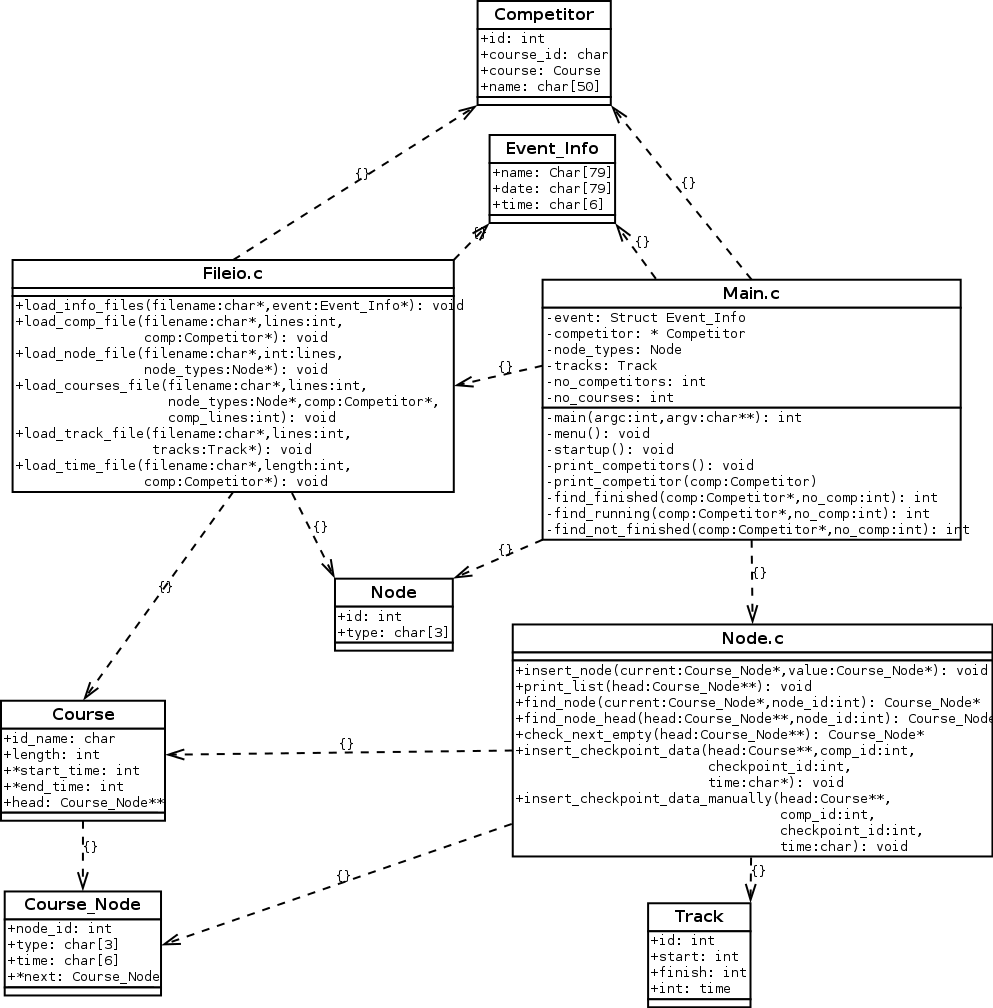
\includegraphics[height=6in,width=6.75in]{../diagrams/module-diagram.png}
	\newpage
	\hspace{-1in}
	\section{Relational Diagram}
	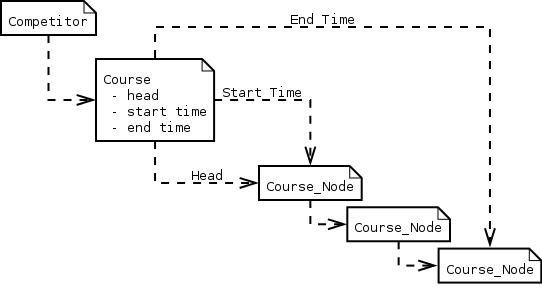
\includegraphics[scale=0.75]{../diagrams/description-of-inheritance.png}
\end{appendices}

\end{document}

